\chapter{Permission implementations in other applications}
As previously mentioned, most implementations for permissions in other web based collaborative content viewing applications are too simplistic and don't provide the user with a complete control over the actions another user takes or the influence they can have on objects. 

\section{Google Drive}
One of the most popular systems for sharing files between users is Google Drive.
Google Drive introduces three ways of sharing a file or a folder with other users:
sharing via contact, sharing via a link, or publishing.

However, associated with these three types of sharing files or folders, a user can set three types of permissions on the files they wish to share: can edit, can view, or can comment. \cite{googleDrivePermission:1}

The "can edit" permission means that the user that gets access to the resource will be able to edit the content of the resource in its entirety.

The "can view" permission is just a read-only permission, thus the user is not allowed to modify the file or folder they have access to.

The "can comment" permission means that the user gets access to Google Drive's comment section and can leave comments regarding the contents of a document.

Although this system is very simple to use it comes with a few drawbacks. There are a few scenarios where sharing documents with the proper permission might cause be an issue. 

\begin{figure}[htbp]
	\centering
		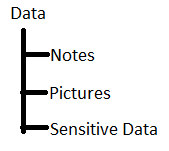
\includegraphics[scale=0.85]{./figures/chapter2/google_drive_file_structure.png}
	\caption{Hard to express file structure}
	\label{FigDriveBadScenario}
\end{figure}

Consider the file structure as shown in figure \ref{FigDriveBadScenario}, assume that the user wants to give access to the folder called "Data" to another user. Currently if the user wants to protect the folder called "Sensitive Data", the only way to do that would be to to share "Notes" and "Pictures" individually without exposing the whole "Data" folder. For this example doing that might work, but once we add a lot of other folders, the whole situation becomes very tedious.

\section{Unix systems}
Although not an online system, unix systems have a very good way of dealing with permissions which is worth going over. The core premise of the unix permission system is that permissions are divided into 3 actions: read, write, execute, along 3 subjects, the owner, the group and other users. 

Alongside all of these, unix systems also provide a so-called "god" role, the root role, which has access over every file and folder, and they can freely execute any command, which involves tinkering with the permissions of other users, groups, files, or folders. In actuality the "root" user is one of the most targeted place of attack, because if a malicious person gains access to the root account, they can do anything in the system.

The problem unix system have with their permission is, again, the lack of granularity. Even though they provide access for the owner, the group, and other users, the fact that you can only control access to one owner, and to one group can lead to issues.

\begin{figure}[htbp]
	\centering
		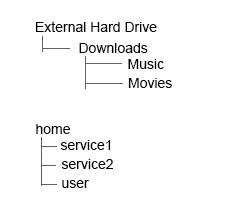
\includegraphics[scale=0.75]{./figures/chapter2/unix_file_structure.png}
	\caption{Complex file structure}
	\label{FigUnixBadScenario}
\end{figure}

Let's take the file structure expressed in \ref{FigUnixBadScenario} as an example. The system has 3 roles: a role for the user --- the owner of the system --- and 2 other roles representing services that are running on the system. Due to security reasons, the services run in their own separate roles.

\begin{table}[htbp]
	\begin{center}
		\begin{tabular}{|p{40pt}|p{220pt}|p{120pt}|}
			\hline User name  &  Access &  Description \\
			\hline 
			\hline user & Everything from the External Hard Drive & The user of the system \\
			\hline service1 & Music & - \\
			\hline service2 & Movies & - \\
			\hline
		\end{tabular}
	\end{center}
	\caption{User roles and permissions}
	\label{UnixRolesAndPerms}
\end{table}

Taking the permissions as described in \ref{UnixRolesAndPerms}, the first role, the user wants complete access ove the external hard drive. The second role, "service1" wants access to just the "Music" folder, without knowing about the existence of the "Movies" folder. And finally the third role "service2" wants access to the "Movies" folder without knowing about the existence of the "Music" folder. 

With just these three roles, the permission scheme proposed is easily achievable as described in \ref{UnixRolesAndPerms2}.
\begin{table}[htbp]
	\begin{center}
		\begin{tabular}{|p{80pt}|p{80pt}|p{80pt}|p{50pt}|}
		\hline Folder & Owner & Group & Other \\
		\hline
		\hline External HDD & user - rw & user - rw & - \\
		\hline Music & user - rw & service1 - rw & - \\
		\hline Movies & user - rw & service2 - rw & - \\
		\hline
		\end{tabular}
	\end{center}
	\caption{User roles and permissions}
	\label{UnixRolesAndPerms2}
\end{table}

The first column represents the folder. The second column represents who the owner is, and the "rw" represents that they have read write access. The third column represents what the group is, and the "rw", again represents that they have read write access. For the sake of example and simplicity the "execute" permission will be left out. The other column represents what permissions other users have, i.e the ones that aren't the owner or are part of the group.

With this permission schema, the user, being the owner of the "External HDD" folder has access over it and all of its subfolders. The role "service1" has access to the "Music" folder, but because the "Music" folder has no read or write permission specified for "others" that means that it can not be accessed by "service2". The same idea was applied to the "Movies" folder, and for the role "service2". 

Even though this is a fairly simple example, the structure of the permission system is a bit cluttered and hard to manage, but in the end it does represent the file structure aforementioned.

The problem with this rises once we introduce more users and more folders.

\begin{figure}[htbp]
	\centering
		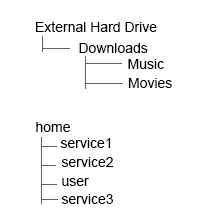
\includegraphics[scale=0.75]{./figures/chapter2/unix_file_structure_2.png}
	\caption{Example bad scenario for unix}
	\label{FigUnixBadScenario2}
\end{figure}

As shown in figure \ref{FigUnixBadScenario2}, the file structure remains the same but a single role has been added. In this case the role "service3" can be seen as a file sharing service such as sambashare. The role "service3" requires complete access over the whole directory that is "Downloads", but no other directories on the External Hard Drive.

Due to the fact that the unix system provides control over a single role, a single owner, and all other users, there is no way of achieving this file structure, and this permission structure, without having to change the structure of the files.
